\chapter{Sistema em Operação}
\label{chap5}


\section{Jovens Gênios Provedor de Conteúdo LTDA}

A Jovens Gênios surgiu em 2016 com Fernando Costa, aluno da Escola de Química da UFRJ e apaixonado por Educação, procurando soluções de ensino extracurriculares engajantes para seus irmãos mais novos. Seguindo uma lógica "efetual"[1] 
Effectuation: Elements of Entrepreneurial Expertise
, não satisfeito com as soluções existentes,desenvolveu plataformas de apoio ao processo de ensino-aprendizagem embrionárias, tendo os irmãos como primeiros usuários.
Junto com o antigo colega Bernard Caffé, que compartilhava a paixão por educação, tendo experiência como professor e com o estudo de Metodologias Ativas de aprendizado, fundaram a empresa Jovens Gênios, tendo escolas de bairro como seus primeiros clientes.

A experiência foi bem sucedida, sendo hoje, seis anos depois, utilizada por centenas de milhares de usuários/alunos de todo o Brasil, os quais registraram através das plataformas Jovens Gênios centenas de milhões de respostas em questões.

\section{Modelagem do Domínio}

O caso de uso da Jovens Gênios inclui nós das estruturas escolares (Redes de ensino, Escolas, Turmas, Alunos, Professores, Gestores), nós do conteúdo gerado pela empresa (Questões, Resumos, Tópicos, Cursos, Disciplinas), nós das atividades que acontecem nas plataformas (Desafios, Tarefas, Provas Somativas, Provas Diagnósticas, Batalhas, Campeonatos, Aulas Invertidas), e, principalmente, os nós referentes às respostas dos alunos, que conectam o aluno à questão e ao contexto da atividade que levou o aluno àquela questão.

A estrutura em árvore dos tópicos e da estrutura escolar, assim como a facilidade de realizar a manutenção e desenvolver novas funcionalidades com as ferramentas disponíveis, foram os fatores determinantes para a escolha de um banco em grafo.

\section{Solução para Supernós}

Supernós são nós que possuem muitos relacionamentos relativos ao resto da rede. Tais nós podem surgir de maneira natural dada uma rede densamente conectada, porém podem causar problemas para o sistema gerenciador do banco de dados do Neo4j.

O driver disponível da Neo4j, apesar de conter e permitir múltiplos acessos de leitura simultâneos ao banco de dados, bloqueia os nós referentes quando executa uma escrita, como por exemplo uma conexão de um nó com outro.
Quando múltiplos usuários simultâneos realizam ações repetitivas que geram nós que se conectam sempre ao mesmo nó, temos impacto no tempo de resposta senão falha crítica do banco de dados.

Encontramos tais problemas em um caso de um Desafio aberto à todos os alunos da plataforma por um tempo limitado. Nesse período, todas as respostas à questões geradas na plataforma eram conectadas ao mesmo desafio. A solução implementada para diminuir o acesso mútiplo de escrita ao mesmo nó foi introduzir um nó intermediário entre o aluno e um Desafio no momento que é liberado à ele, e as respostas (e qualquer outra da interação entre o Desafio e o Aluno) são conectadas nesse nó intermediário, ao invés de diretamente no Desafio em si.

    \begin{figure}[H]
        \centering
        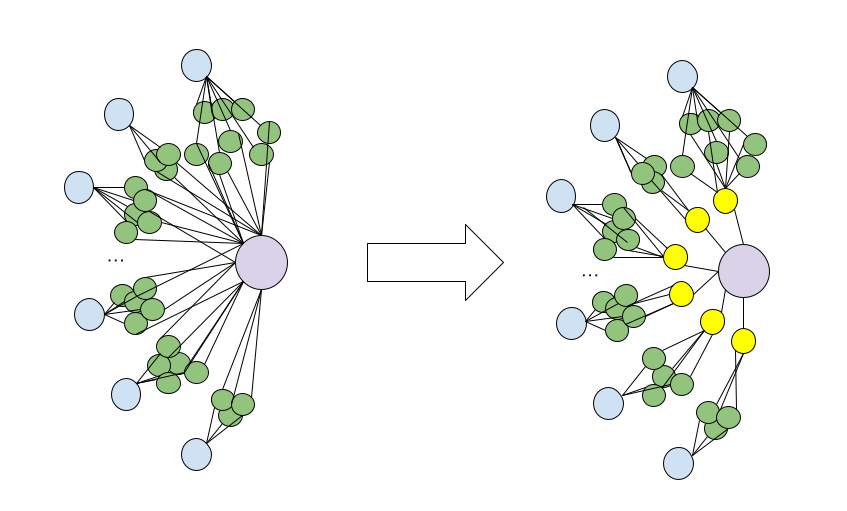
\includegraphics[width=1.0\linewidth]{Imagens/chap05/AssignedContext.png}
        \caption{Alunos, respostas e Desafio conectados diretamente, e através de um nó intermediário}
        \label{fig:profile-exemple}
    \end{figure}
Dessa forma, cada aluno (nó que gera os outros nós) tem um nó para si, e as operações de escrita bloqueantes antes executadas no nó central são distribuídas entre os nós intermediários.

Tal modelagem impactou o sistema "Admins", ficando menos intuitivo a navegação entre o perfil do Aluno e suas Atividades (não só desafios, qualquer atividade que poderia ter uma quantidade significativa de alunos simultâneos online). Decidimos que o ideal era esconder o nó intermediário da navegação, e o clique em um elemento do nó intermediário na tabela redireciona o usuário diretamente ao perfil da atividade (ou aluno) do outro lado. As respostas sendo resolvidas por um cypher personalizado ao schema nos dois lados.

\section{Papeis dos Usuários do sistema ``Admins''}

Os seguintes perfis de colaboradores são usuários do sistema ``Admins'' na Jovens Gênios:

\begin{itemize}
    \item Educacional (Responsáveis pelo contato direto com as escolas e definição das turmas)
    \item Suporte (Contato com alunos e professores para esclarecer dúvidas e mapear eventuais problemas)
    \item QA (Controle de qualidade e interface com os desenvolvedores)
    \item Desenvolvedores (Visualizar e realizar eventuais manipulações no banco de dados)
\end{itemize}

